\let\negmedspace\undefined
\let\negthickspace\undefined
\documentclass[journal]{IEEEtran}
\usepackage[a5paper, margin=10mm, onecolumn]{geometry}
%\usepackage{lmodern} % Ensure lmodern is loaded for pdflatex
\usepackage{tfrupee} % Include tfrupee package

\setlength{\headheight}{1cm} % Set the height of the header box
\setlength{\headsep}{0mm}     % Set the distance between the header box and the top of the text

\usepackage{gvv-book}
\usepackage{gvv}
\usepackage{cite}
\usepackage{amsmath,amssymb,amsfonts,amsthm}
\usepackage{algorithmic}
\usepackage{graphicx}
\usepackage{textcomp}
\usepackage{xcolor}
\usepackage{txfonts}
\usepackage{listings}
\usepackage{enumitem}
\usepackage{mathtools}
\usepackage{gensymb}
\usepackage{comment}
\usepackage[breaklinks=true]{hyperref}
\usepackage{tkz-euclide} 
\usepackage{listings}
% \usepackage{gvv}                                        
\def\inputGnumericTable{}                                 
\usepackage[latin1]{inputenc}                                
\usepackage{color}                                            
\usepackage{array}                                            
\usepackage{longtable}                                       
\usepackage{calc}                                             
\usepackage{multirow}                                         
\usepackage{hhline}                                           
\usepackage{ifthen}                                           
\usepackage{lscape}
\begin{document}

\bibliographystyle{IEEEtran}
\vspace{3cm}

\title{12.6.5.2.3}
\author{EE24BTECH11019 - Dwarak A}
% \maketitle
% \newpage
% \bigskip
{\let\newpage\relax\maketitle}

\renewcommand{\thefigure}{\theenumi}
\renewcommand{\thetable}{\theenumi}
\setlength{\intextsep}{10pt} % Space between text and floats


\numberwithin{equation}{enumi}
\numberwithin{figure}{enumi}
\renewcommand{\thetable}{\theenumi}

\textbf{Question:}

Solve the following pair of linear equations,
\begin{align}
    \frac{3x}{2} - \frac{5y}{3} &= -2\\
    \frac{x}{3} + \frac{y}{2} &= \frac{13}{6}
\end{align}
\textbf{Solution:}
\newline
Let
\begin{align}
    \vec{x} = \myvec{x\\y}
\end{align}
Expressing the system in matrix form,
\begin{align}
    \myvec{\frac{3}{2} & \frac{-5}{3}\\ \frac{1}{3} & \frac{1}{2}}\vec{x} &= \myvec{-2\\\frac{13}{6}} \\
    \myvec{9 & -10 \\ 2 & 3}\vec{x} &= \myvec{-12 \\ 13} \\
    A\vec{x} &= \vec{b}
\end{align}
Any non-singular matrix $A$ can be expressed as a product of a lower triangular matrix $L$ and an upper triangular matrix $U$, such that
\begin{align}
    A &= LU\\
    \implies LU\vec{x} &= \vec{b}
\end{align}
$U$ is determined by row reducing $A$ using a pivot,
\begin{align}
    \myvec{9 & -10\\2 & 3} \xrightarrow{R_2 \to R_2 - \frac{2}{9}R_1} \myvec{9 & -10\\0 & \frac{47}{9}}
\end{align}
Thus
\begin{align}
    U = \myvec{9 & -10\\0 & \frac{47}{9}}
\end{align}
Let 
\begin{align}
    L = \myvec{1 & 0\\l & 1}
\end{align}
$l$ is the multiplier used to zero out $a_{21}$ in $A$.
\begin{align}
    L = \myvec{1 & 0\\ \frac{2}{9} & 1}
\end{align}
This $LU$ decomposition could also be computationally found using Doolittle's algorithm. The update equation is given by,
\begin{align}
    U_{ij} &= \begin{cases}
        A_{ij} & \quad i = 0\\
        A_{ij} - \sum_{k = 0}^{i - 1} L_{ik} U_{kj} & \quad i > 0
    \end{cases}\\
    L_{ij} &= \begin{cases}
        \frac{A_{ij}}{U_{jj}} & \quad j = 0, U_{jj} \neq 0\\
        \frac{A_{ij} - \sum_{k = 0}^{j - 1} L_{ik} U_{kj}}{U_{jj}} & \quad j > 0
    \end{cases}\\
\end{align}
Now,
\begin{align}
    A = \myvec{9 & -10 \\ 2 & 3} = \myvec{1 & 0 \\ \frac{2}{9} & 1}\myvec{9 & -10 \\ 0 & \frac{47}{9}}
\end{align}
Now we can get the solution to our problem by the two step process,
\begin{align}
    L\vec{y} = \vec{b}\\
    U\vec{x} = \vec{y}
\end{align}
Using forward substitution to solve the first equation,
\begin{align}
    \myvec{1 & 0 \\ \frac{2}{9} & 1}\myvec{y_1 \\ y_2} &= \myvec{-12 \\ 13}\\
    \myvec{y_1 \\ y_2} &= \myvec{-12 \\ \frac{47}{3}} 
\end{align}
Now using back-substitution for the second equation,
\begin{align}
    \myvec{9 & -10 \\ 0 & \frac{47}{9}}\myvec{x_1 \\ x_2} &= \myvec{-12 \\ \frac{47}{3}}\\
    \myvec{x_1 \\ x_2} &= \myvec{2 \\ 3}
\end{align}

\begin{figure}[ht]
    \centering
    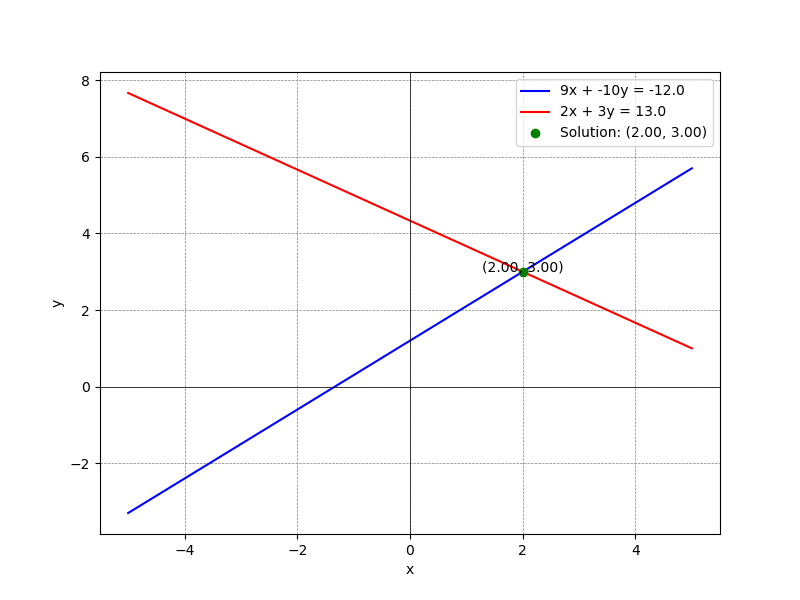
\includegraphics[width=\columnwidth]{figs/plot.png}
    \caption{Plot of local maximum and minimum}
    \label{fig:Plot1}
    \end{figure}
\end{document}}
